\section{Passing metadata between nodes}
To implement the \textit{tainting dependencies method}, it is necessary to pass
several types of metadata upwards when parsing the syntax tree, such as
variable references and flags to indicate singleton nodes. Additionally, the
operator tree which is being built bottom-up (as described earlier in section
\ref{sect:impl:construct_mql}) is also required to be passed upwards. 

This is achieved through the \texttt{TaverseReturn}, which models a return type
when visiting nodes in the syntax tree. That is, the visitor methods are
responsible of 1) visiting any child nodes, and 2) returning an instance of the
\texttt{TraverseReturn} class based on what was returned from the child nodes,
if anything.

\subsection{The TraverseReturn class}
The class diagram for the \texttt{TraverseReturn} class is shown in figure
\ref{fig:impl:meta:traverse_uml}. Note the flag to indicate if the current
context is a singleton, the reference to an MQL operator tree (which is being
built bottom-up), and a reference to a set of ``variable references'' -- that
is, variables in the XQuery query that are read but never altered.

\begin{figure}[!htp]
\begin{center}
  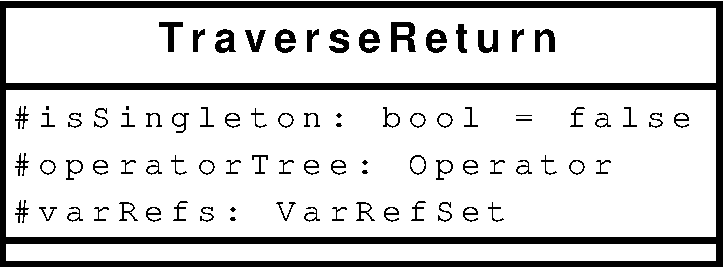
\includegraphics[scale=0.5]{diagrams/traversereturn_uml}
  \caption{TraverseReturn class diagram}
  \label{fig:impl:meta:traverse_uml}
\end{center}
\end{figure}

The \texttt{TraverseReturn} class is, as mentioned, used in the visitor when
visiting nodes in the abstract syntax tree (see section
\ref{sect:impl:context_sens_visitor}). A typical use case is shown in figure
\ref{fig:impl:meta:traverse_usage_ex}, which is an excerpt from the
implementation.

\subsection{Variable references}
Variable references, as described in section \ref{sect:trans:TD:basics}, are
passed upwards together with the MQL operator tree being built during the syntax
tree parsing process. These sets of references are integral to the
\textit{tainting dependencies method}.

The class diagram for the \texttt{VarRefSet} class and its associated
\texttt{VarRef} class is shown in figure \ref{fig:impl:meta:varrefset_uml}.

\begin{figure}[!htp]
\begin{center}
  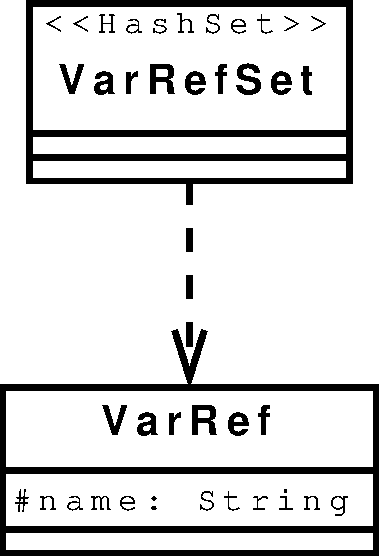
\includegraphics[scale=0.5]{diagrams/varrefset_uml}
  \caption{\texttt{VarRefSet} and \texttt{VarRef} class diagram}
  \label{fig:impl:meta:varrefset_uml}
\end{center}
\end{figure}

When a variable is encountered during the parse process, and the variable is
being ``read'' and not altered (i.e set to a value), the variable reference is
added to the current set of variable references, which is a part of the resulting
\texttt{TraverseReturn} instance which should be returned from the visitor.
The example in figure \ref{fig:impl:meta:var_ref_ex} shows the variable \$a
being ``read'', in which case it is counted as a variable reference.

\begin{figure}[!htp]
\begin{center}
\begin{Verbatim}
for $i in (1,2,3) return $a
\end{Verbatim}
  \caption{Example of the variable \$a being ``read''}
  \label{fig:impl:meta:var_ref_ex}
\end{center}
\end{figure}

\subsection{Singleton nodes}

\subsection{Example of usage}

\begin{figure}[!htp]
\begin{center}
\begin{Verbatim}
    public TraverseReturn visitIntegerLiteral(XQFTTree tree) {

        StringBuffer b = new StringBuffer();
        b.append("name:=[value],");
        b.append(tree.getText());
        
        Make make = new Make(b.toString());

        TraverseReturn tr = new TraverseReturn();
        
        tr.setSingleton(true);
        tr.setOperatorTree(make);

        return tr;
    }
\end{Verbatim}
  \caption{TraverseReturn usage example}
  \label{fig:impl:meta:traverse_usage_ex}
\end{center}
\end{figure}

In this example an integer literal node is visited (a node that simply holds an
integer). A \texttt{make()} MQL operator as well as a new
\texttt{TraverseReturn} instance is created. The \texttt{make()} operator is
then appended to the \texttt{TraverseReturn} instance, and the
\textit{isSingleton} flag is set to \textit{true}.